\subsection{Conditional Independence}
\begin{frame}{Conditional Independence}
	\begin{columns}
		\begin{column}{0.49\textwidth}
\begin{definition}[Independence of States]
	We say a state $f:I\rightarrow X\otimes Y$ exhibits $$X \bot Y$$ if it can be factored as
	\begin{equation*}
		\tikzfig{state-independence}
	\end{equation*}
\end{definition}
		\end{column}
		\pause
		\begin{column}{0.49\textwidth}
	\begin{example}[$\mathsf{FinStoch}$]
		\begin{equation*}
		f(x,y) = g(x)h(y)
		\end{equation*}
		\begin{figure}
		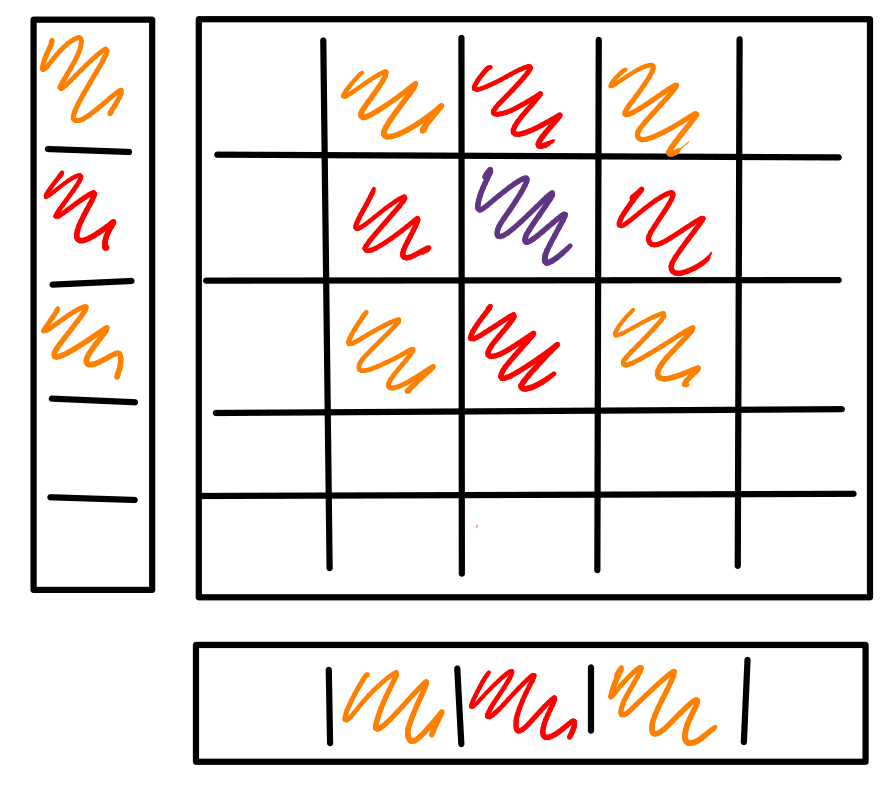
\includegraphics[align=c, scale=0.15]{graphics/finstoch-independent}
		\end{figure}
	\end{example}
		\end{column}
	\end{columns}
\end{frame}

\begin{frame}{Conditional Independence}
	\begin{columns}
		\begin{column}{0.49\textwidth}
	\begin{definition}[Independence Conditioned on an Input]
		A morphism $f:A\rightarrow X\otimes Y$ exhibits $$X \bot Y \parallel A$$ if it can be factored as
		\begin{equation*}
			\tikzfig{input-independence}
		\end{equation*}
	\end{definition}
		\end{column}
		\pause
		\begin{column}{0.49\textwidth}
	\begin{definition}[Independence Conditioned on an Output]
		A morphism $f:I\rightarrow X\otimes B \otimes Y$ exhibits $$X \bot Y\ |\ B$$ if it can be factored as
		\begin{equation*}
			\tikzfig{output-independence}
		\end{equation*}
	\end{definition}
		\end{column}
	\end{columns}
\end{frame}

\begin{frame}{Conditional Independence}
	\begin{definition}[General Conditional Independence]
		A morphism $f:A\rightarrow X\otimes B \otimes Y$ exhibits $$X \bot Y\ |\ B \parallel A$$\\ if it can be factored as
		\begin{equation*}
			\tikzfig{combined-independence}
		\end{equation*}
	\end{definition}
\end{frame}

\subsection{Conditionals}
\begin{frame}{Conditionals}
	\begin{definition}
		For a morphism $f:A\rightarrow X\otimes B$, a conditional $f_{|B}: A\otimes B \rightarrow X$ is any morphism that satisfies
		\begin{equation*}
			\tikzfig{conditional}
		\end{equation*}
	\end{definition}
\end{frame}

\begin{frame}{Conditionals}
	\begin{columns}
		\begin{column}{0.49\textwidth}
	\begin{example}[$\mathsf{FinStoch}$]
		\begin{equation*}
			f_{|B}(y|b) = \frac{f(y,b)}{\sum_y f(y,b)}
		\end{equation*}
			\begin{center}
		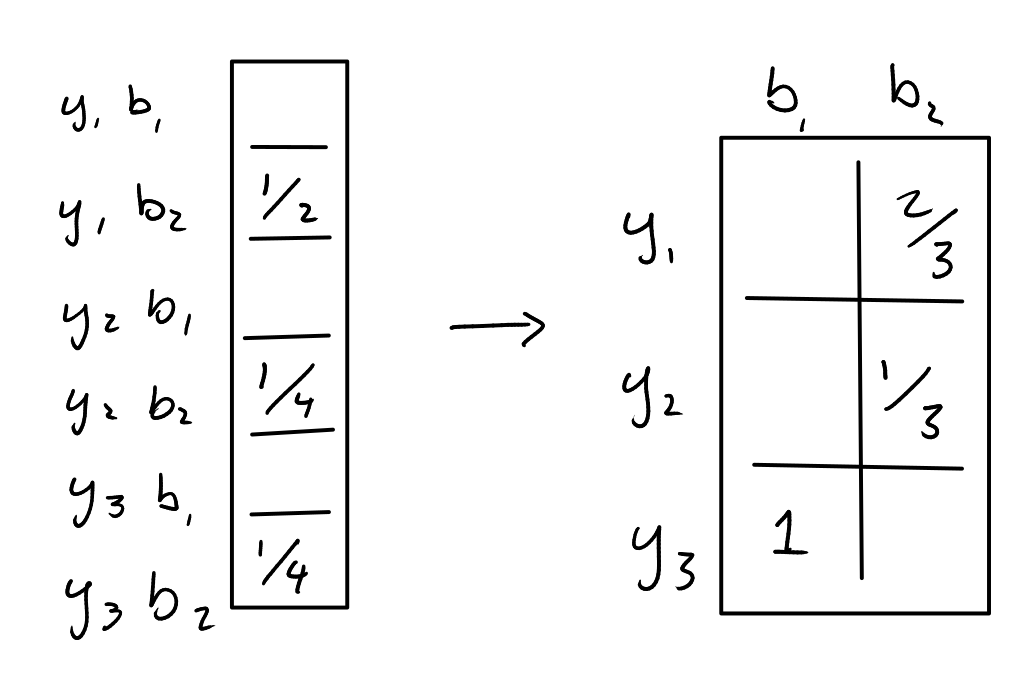
\includegraphics[align=c, scale=0.15]{graphics/finstoch-conditional}
		\end{center}
	\end{example}
		\end{column}
		\pause
		\begin{column}{0.49\textwidth}
	\begin{example}[Independent morphisms are not correlated!]
		If $X\bot B \parallel A$, then one valid conditional is
		\begin{equation*}
			\tikzfig{conditional-independent}
		\end{equation*}
	\end{example}
		\end{column}
	\end{columns}
\end{frame}

\begin{frame}{Conditionals}
		Conditionals may not exist. Eg., $\mathsf{Stoch}$ does not have all conditionals. Many categories do have all conditionals, however:
		\begin{itemize}
			\item All deterministic Markov categories
			\item $\mathsf{BorelStoch}$
			\item $\mathsf{FinStoch}$
			\item $\mathsf{FinSetMulti}$
			\item $\mathsf{Gauss}$
		\end{itemize}
\end{frame}

\begin{frame}{Conditionals}
	\begin{columns}
		\begin{column}{0.49\textwidth}
	\begin{definition}[Almost Sure Equality]
		$f_1$ and $f_2$ are $g$-almost surely equal if
		\begin{equation*}
			\tikzfig{almost-surely}
		\end{equation*}
		We write this as $f_1 =_{g-a.s.} f_2$
	\end{definition}
		\end{column}
		\pause
		\begin{column}{0.49\textwidth}
	For $f:A\rightarrow X\otimes B$, $f_{|B}$ is almost surely unique with respect to:
		\begin{equation*}
			\tikzfig{conditional-uniqueness}
		\end{equation*}
		\end{column}
	\end{columns}
\end{frame}

\begin{frame}{Conditionals}
	\begin{columns}
		\begin{column}{0.29\textwidth}
	\begin{definition}[Dashed-Box Notation]
		\begin{equation*}
			\tikzfig{dashed-box-notation}
		\end{equation*}
	\end{definition}
		\end{column}
		\pause
		\begin{column}{0.69\textwidth}
	\begin{block}{Rewrite Rules}
		\begin{equation*}
		\tikzfig{conditional-rewrites}
		\end{equation*}
	\end{block}
		\end{column}
	\end{columns}
\end{frame}

\begin{frame}{Conditionals}
	\begin{columns}
		\begin{column}{0.49\textwidth}
	\begin{definition}[Bayesian Inverse]
		For $f:X\rightarrow Y$, its Bayesian inverse with respect to state $p$ on $X$ is
		\begin{equation*}
			\tikzfig{bayesian-inverse}
		\end{equation*}
	\end{definition}
		\end{column}
		\pause
		\begin{column}{0.49\textwidth}
		The Bayesian inverse satisfies
		\begin{equation*}
			\tikzfig{bayes-equation}
		\end{equation*}
		\pause
			\begin{example}{$\FinStoch$}
				\begin{equation*}
					f_p^{\dagger}(x|y) =
					\frac{f(y|x)p(x)}{\sum_x f(y|x)p(x)}
				\end{equation*}
			\end{example}
		\end{column}
	\end{columns}
\end{frame}
